%!TEX root = thesis.tex

\chapter{Summary}
\label{chap:summary}

A number of statements were examined throughout the preceding chapters.
-there is a need for increased audience understanding within live coding
-there is a need for increased audience enjoyment within live coding
-there is a need for increased live coder understanding within live coding
-there is a need for increased live coder enjoyment within live coding
-there is a measurable effect on enjoyment with the visualisations compared to without
-there is a measurable effect on understanding with the visualisations compared to without

-visualisations have a place in live coding
-visualisations have a place in understanding the coding process
-visualisations can communicate the coding process more effectively than without
-visualisations have a place in understanding code structures

-qualitative factors seemed to contribute more to the appreciation of the visualisations. People tended towards suggesting that the visualisations should match the music more than the code?

{\color{red} state their validity here}

\afterpage{
\begin{figure}
  \centering
  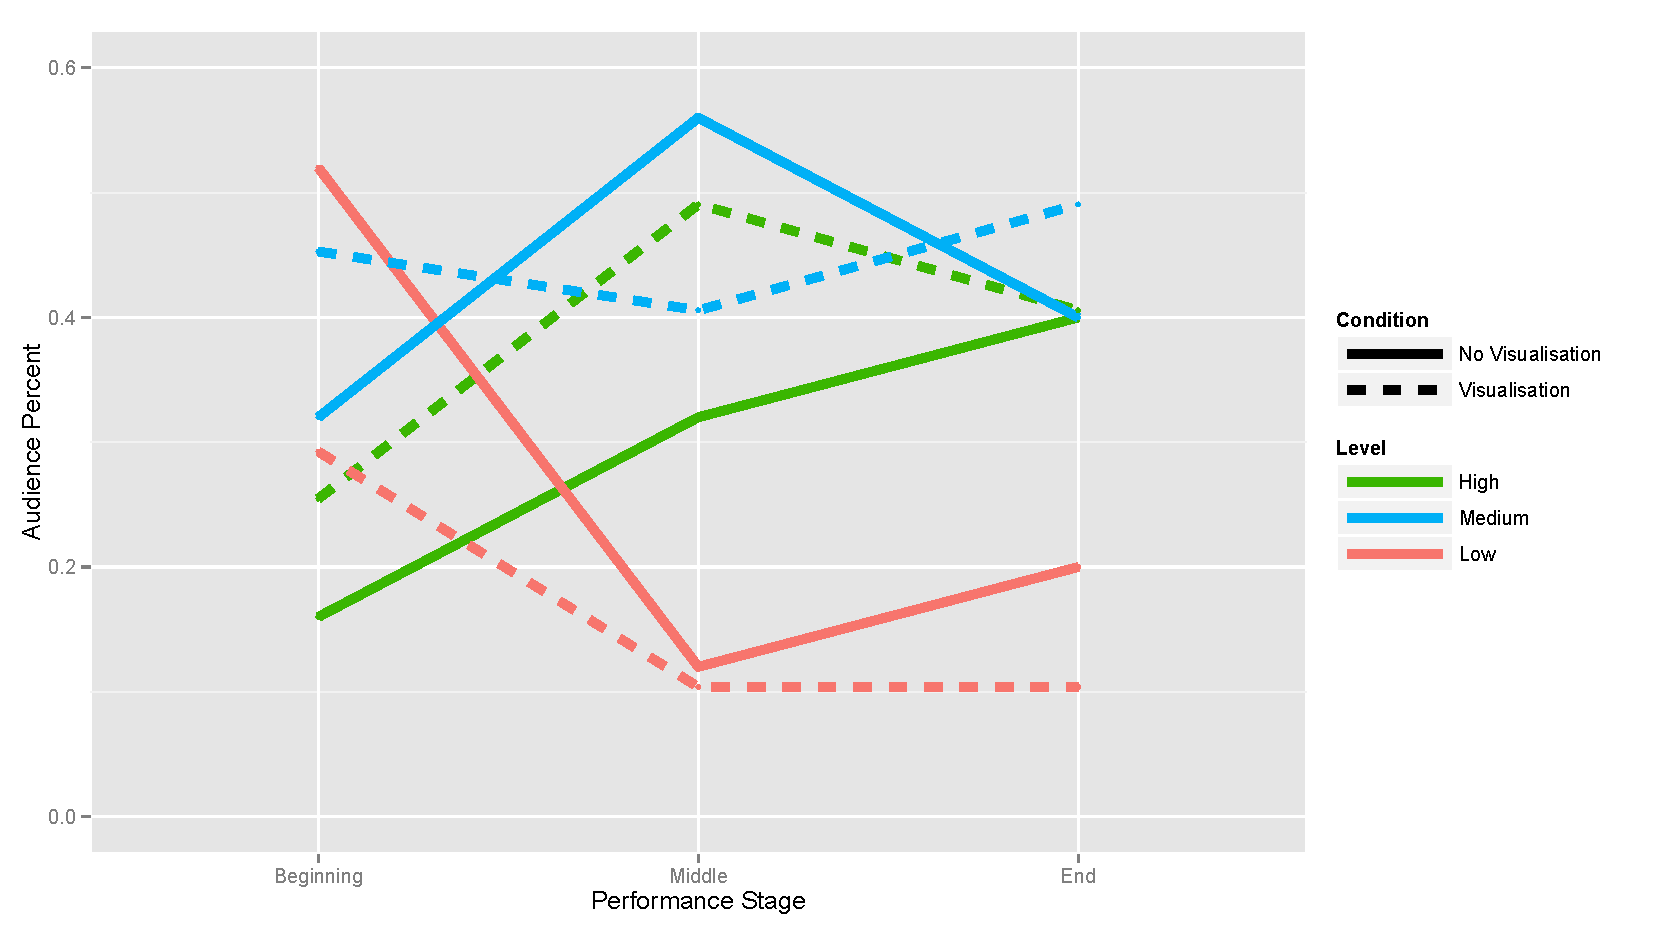
\includegraphics[width=\columnwidth]{../images/graphs/enjoyment-final.pdf}
  \caption{Aggregate comparison of enjoyment within live coding with and without visualisations including results from the intial user study and the follow-up user study.}
  \label{fig:enjoyment-final}
\end{figure}

\begin{figure}
  \centering
  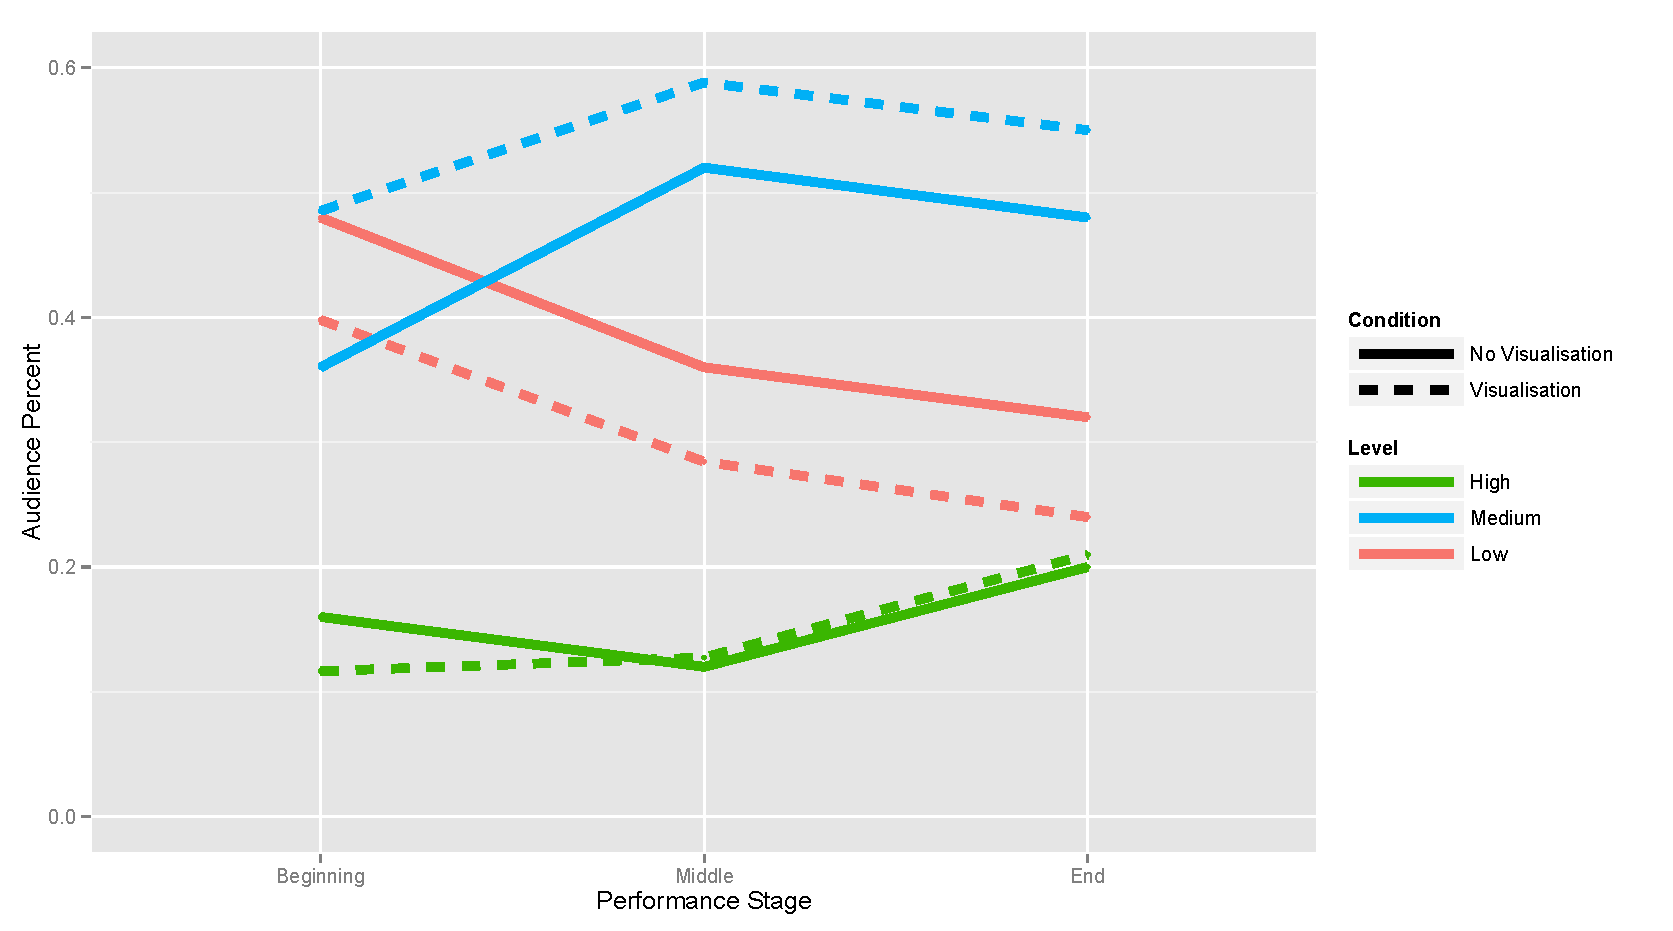
\includegraphics[width=\columnwidth]{../images/graphs/understanding-final.pdf}
  \caption{Aggregate comparison of understanding within live coding with and without visualisations including results from the intial user study and the follow-up user study.}
  \label{fig:understanding-final}
\end{figure}
\clearpage}

From presentation (for Figure~\ref{fig:enjoyment-final}):

[results of this study and the results of previous user study gave rise to the following….]
this graph shows the percent of the audience reporting their levels of enjoyment over the three stages of the performance for the two conditions of “no visualisation” and “with visualisation” 
the no visualisation condition is marked as a solid line
the visualisation condition is marked as a dotted line
the percent of the audience reporting high is marked in green, reporting medium is marked in blue and reporting low is marked in red
a smaller percentage of the low group and a larger percentage of the high group would be desirable

- for example, during the beginning of the performance, for the visualisation condition, 30% of the audience stated that they had low enjoyment while for the no visualisation, 50% of the audience stated that they had low enjoyment

this graph shows an overall increase in enjoyment consistently throughout the performance
increase in a high level of enjoyment with the visualisation, particularly during the middle of the performance
in summary, these results indicate that there is a clear shift upwards in enjoyment throughout the performance, with the visualisations always performing equal or better than the no visualisation condition

From presentation (for Figure~\ref{fig:understanding-final}):

this graph is for understanding and is a similar format to the previous
coloured lines show percent of audience with that level of understanding

shows an increase in the percent reporting medium understanding with the visualisation compared to without… 
visualisations appears to help audiences reporting low understanding
however, little impact on the percent reporting high levels of understanding
-  in summary, it shows a consistent increase throughout the performance for all except those with high understanding




\section{Contributions}

Throughout the investigation of the application of software visualisations to live coding a number of contributions to the field have been identified. This section outlines these contributions.

Principally, a method of software visualisation has been identified and evaluated. Up to now there has been no attempt to evaluate visualsations within the space of live coding. The method of process-driven visualisation identified has included a combination of static and dynamic code analysis and presentation to audiences during live coding performances.

Through the development of the software visualisation prototypes, a strategy for developing visualisations using a software engineering approach has been identified. This approach has involved collaboration with a musical artist with the application of a software engieering design, iteration and validation approach through a variety of field and user studies.

The development of the software visualisation prototype and the application to the live coding space have allowed the development of a method of evaluating software visualisations within a live performance space. The more general implications of this method of visualisation evaluation may be useful in the evaluation of software developed for large audiences and audiences observing an individual developing software.

A conference short paper discussing the prototype and evaluation methodology has been accepted to the OzCHI conference entitled ``Visualising a Live Coding Arts Process''. Anonymous references indicated that ``the questions raised are worthwhile and interesting'', ``the paper describes interesting work'' and that it is ``an interesting paper, and certainly a novel contribution''.

% Finally, a novel approach to visualising the programming process has been developed.

Updated software visualisation taxonomy built on the existing software visualisation frameworks...

Method of developing process driven software visualisation for live coding...

Process-driven software visualisation showing software as it is being developed (live, as in live-coding)...

Evaluation of a process-driven software visualisation...

Contribution to live coding process and outcome... A multi-disciplinary approach, implementation and evaluation of a software application.

Discuss recommendations?...

``...methodological issues have to be studied further. This concerns questions like how to design visualizations and how to measure and evaluate the effectiveness of various solutions.''~\cite{VanWijk2005} A methodology for visualisation design has been developed.


\section{Limitations}

Despite significant contributions in the space of visualisation methodology and software visualisation design, development and evaluation, some limitations with the process have been identified.

limitations to evaluation methodlogy
-type of language may affect understanding. Imperitive vs functional etc.

limitations to generalisation
-how wide can the results of this study be generalised outside of the field of live coding.

limitations to assumptions
-understanding and enjoyment are not necessarily entirely independent. enjoyment may contribute to understanding. understanding may contribute to enjoyment.

limitations to visualisation methodology

\section{Future Work}

-two screens

Software visualisations that interact directly with the programmer are yet to be adopted into mainstream development. Similarly, the visualisation of the live coding process has not yet been adopted into live coding performances.

From presentation:

 just the beginning of what is possible within this area
future work will:
-  identify what audiences really find interesting and worthwhile within visualisations of live coding
develop live coded visuals - much potential to harness the data that has been extracted. it would be worthwhile to take these ideas, further integrating them into the live coding process or introducing them to other software processes using the methodology identified
 further develop the methodology
identified two dimensions of enjoyment and understanding, and three phases of the performance that are of interest: the beginning, middle and end. it would be worthwhile to further articulate these concepts
could include more comprehensive user studies... clear up some of the technical challenges encountered... for example one idea identified would be using two projectors, one with source code, one with the visualisation



\subsection{Software Engineering}


\subsection{Live Coding}


\subsection{Evaluation Methodology}

The evaluation methodology described...



Aesthetic elements of the software...

Didactic elements of the software...

Future of visualisations in live coding...

Application to software engineering practice...

Application to the arts...

Visualisation as a means to communicate the coding process...

Visualisation as a means to more effective coding...

More general application to software development


